\documentclass{article}
\usepackage{graphicx} % Required for inserting images
\graphicspath{{images/}} %configuring the graphicx package
\usepackage{listings}
\usepackage{xcolor}
\usepackage[utf8]{inputenc}
\usepackage{babel}
\usepackage[margin=2.5cm]{geometry}
\usepackage{todonotes} %for to do notes
\usepackage{enumitem} %for customizable enumerations
\usepackage{soul}
\usepackage{xcolor}  % Load the xcolor package
\usepackage{caption}
\usepackage{array}
\usepackage[utf8]{inputenc}
\usepackage{graphicx}



%definition of variables for uniformity of naming
\newcommand{\admin}{admin }
\newcommand{\admins}{admins }
\newcommand{\adminGroup}{admin group }
\newcommand{\adminGroups}{admin groups }
\newcommand{\participant}{participant }
\newcommand{\participants}{participants }
\newcommand{\group}{groups }
\newcommand{\groups}{groups }
\newcommand{\user}{user }
\newcommand{\users}{users }


%notes: respect the correct formatting of the Latex code in order to increase readability.
% each section should start at the leftmost area of the screen and each subsection should be indented.
%use to do blocks to spot areas that needs further development or examination
%always refer to the sytem as system, not website or other specific names because this will result in a premature desing choice




\title{RASD\\ CodeKataBattles}
\author{Federica Laudizi, Antonio Marusic, Sara Massarelli}
\date{November 2023}

\begin{document}


\maketitle

\tableofcontents


\begin{abstract}
    This Requirements Analysis and Specification Document (RASD) is going to tackle objectives, requirements (functional and non functional) for the project CodeKataBattles.
    
    It will be presented the scope, the functionalities and the domain of such project and we will give a comprehensive overview of the interaction with users and external components and the performance expected from the system.

    This document is going to be a reliable point of reference for developers since it will define clearly the functionalities of the system and it will give precise guidelines during the validation and verification process.

    The profound goal of this document is to give a precise overview of the product to be in order to give the stakeholders a general understanding of usage scenarios and avoiding changes of directions during the design and implementation part of the system development.    
\end{abstract}

\section*{Tasks}

\todo[inline,color=blue!40]{Task 1: come si chiude un torneo?}
\todo[inline,color=green!40]{Task 2: come si chiude una battaglia?}
\todo[inline,color=pink!40]{Task 3: definire bene come uno studente che non appartiene a un tournament può essere invitato a partecipare a una battaglia}
\todo[inline,color=pink!40]{Task 3: possono essere invitati degli student anche a partecipare a un torneo?}
\todo[inline,color=pink!40]{Forse negli state diagram ci starebbe uno che descrive l'evoluzione dello stato di una battle in queste tre fasi: kata battle subsctiprion phase, push phase, consolidation phase}
\todo[inline,color=pink!40]{Abbiamo messo come requirements che gli studenti fanno correttamente il branch della repo?}
\todo[inline,color=pink!40]{come fa il sistema a capire quale branch è di chi?}
\todo[inline,color=pink!40]{può il sistema mandare una eccezione se la branch non è creata corretamente?}
\todo[inline,color=pink!40]{si può settare da github il fatto che la repo non permetta di vedere altri branch rispetto al main a e a quello creato da te?}
\todo[inline,color=pink!40]{gli studenti devono fare un fork, non un branch}
\todo[inline,color=pink!40]{il sistema si accorge dei push solo quando questi vengono fatti sul branch main del fork dello studente}
\todo[inline,color=pink!40]{spiega da qualche parte cos'è un gruppo aperto e uno chiuso}


\section{Introduction} 
    \subsection{Purpose}
        This system allows users to boost their learning by participating in
        code challenges called kata battles organised by teachers or independent tutors.\\

        Such challenges will be part of tournaments so that it is possible for students to compete in multiple katas and seeing their position in a leaderboard of all participants.
        The system allows for the creator of the tournament to define a set of rules regarding the number of participants and the size of the groups of students and it gives the possibility to delegate the creation of the katas and the managing of the tournament also to other teachers.\\

        The system offers a platform integrated with GitHub where teachers can publish the kata and define the test cases that the code provided by the students must pass and assess student's submissions.
        The students on the other hand, can submit their code and see immediately
        its performances. The system assigns a score to each submission
        based on functional and non functional aspects of the code so that
        students can compare their work with other participants.\\
        
        Moreover, the system promotes global participation in kata battles, since it is possible to join battles organised by educators from all around the world.
        It is worth noticing that, not only certified teachers can create tournaments, but also independent tutors, allowing them to engage their students in productive competitions. 
            \subsubsection{Actors definitions}\label{sec:actor_definitions}
                The actors interacting with the system were identified as follows:
                \begin {itemize}
                    \item Guest: someone that accesses the website but is not yet registered to access the functionalities.
                    \item User: is a registered person in the system.
                    \item Admin: teachers, educators or tutors that created the tournament or were invited by the creator as collaborators. Admin users have the privilege for that tournament to manage the its settings and parameters and to generate new kata battles.
                    \item Participant: student within a group. 
                    \item Group: team of students that participants in a tournament.
                \end {itemize}
                For further details on user characteristic refer to section \ref{sec:user_characteristics}.
            \subsubsection{Definitions}
                \begin {itemize}
                    \item Kata battle: a coding exercise where a task is given to the participants and they have to submit their solution through GitHub.
                    \item Tournament: a competition made of a sequence of Kata battles , each contributing to a final score. The score of these battles are then used to establish a leaderboard that ranks the participants.
                    \item Badge: A badge is a collectible award earned when specific predefined conditions are met. There are two types of badges:
                    \begin {itemize} 
                        \item Top-type badges: These are obtained when a participant in a tournament achieves the highest ranking in a specific category. For example, a participant might receive a top-type badge for being the top committer or writing the most time efficient code.
                        \item Boolean-type badges: These are awarded to the first X participants who meet a specific condition defined by administrators. The value of X is set by administrators and represents the number of participants eligible to receive the badge. It could be, for instance, the first 10 participants who complete a certain challenge or meet a particular criterion.
                    \end {itemize}
                \end {itemize}
                    
            \subsubsection{Goals}
                The system must satisfy the following goals:
                \begin{enumerate}[label=\textbf{G\arabic*}:, left=0pt]
                    \item Users can join a tournament.
                    \item Groups can submit their code through GitHub.
                    \item Admins and groups can view the current rank evolving through each battle and tournament.                    
                    \item Participants can see all tournaments currently running.
                    \item Admins can invite collaborators to the tournament that will be considered as admins once they accept the invite.
                    \item Admins can accept user requests to participate in a tournament.
                    \item Admins can create tournaments and battles within them.
                    \item Admins can modify key settings when creating tournaments. These settings can include:  making  the tournament public, set a maximum number of participants, limits on group sizes, or a  duration of each kata battle. 
                    \item Admins can evaluate the work done by students.
                    \item Admins can define badges (e.g., “top committer”)  when they create a tournament. Each badge has a title and one or more rules (i.e., simple Boolean properties) that must be fulfilled to achieve the badge.
                    \item User can see collected badges when they visualize the profile of a student.
                    \item User can request to participate in a tournament.
                    \item Participants can create groups for the battles.
                    \item Participants can invite other students in the tournament to join their group for a battle.
                    \item Participants can accept or refuse the invite to join a group for a battle.
                    \item Participants can join a public group.
                    
                \end{enumerate}
                \todo {to be continued}

    \subsection{Scope}
        here we include an analysis of the world and of the shared phenomena, Acronyms, Abbreviations.

        \subsubsection{World phenomena}
            \begin{enumerate}[label=\textbf{WP\arabic*}:, left=0pt]
                \item User has a GitHub account.
                \item User has a personal computer with internet access.
                \item User has an email account.
                \item User can write code and format it as required
            \end{enumerate}
        \subsubsection{Shared phenomena}
        Controlled by the world and observed by the machine (SPWC).

        \begin{enumerate}[label=\textbf{SPWC\arabic*}:, left=0pt]
            \item Student or Teacher registers in the system.
            \item Student or Teacher logs in the system.
            \item Teacher requests the system to create a new tournament.
            \item Teacher requests the system to create a new kata battle inside a tournament.
            \item Teacher requests the system to set configuration parameters of a tournament he/she is managing.
            \item Teacher requests the system to invite new admins to handle a tournament.
            \item Teacher modifies the score of a group in the consolidation phase of the kata battle.
            \item Teacher accepts or rejects an invitation to an admin group.
            \item Student requests the system to join a tournament.
            \item Student requests the system to join a battle.
            \item Student invites other students to join his group for a battle.
            \item Student modifies the status of the group he is in from open to closed and the other way around.
            \item Student pushes code on the group branch on the GitHub repository.
            \item Student accepts or rejects an invitation to a group.
        \end{enumerate}

        Controlled by the machine and observed by the World (SPMC).

        \begin{enumerate}[label=\textbf{SPMC\arabic*}:, left=0pt]
            \item The system updates the group score.
            \item At the expiry time of the subscription phase of a kata battle, the system removes all the groups that don't match the requirements on the number of participants.
            \item At the expiry time of the subscription phase of a kata battle, after the removal of incomplete groups, the system notifies every participant of the battle and sends a link to the GitHub repository.
            \item In case the tournament is set to open to everyone, the system notifies every student registered on the platform of this event.
            \item The system notifies a student of the invitation in a group.
            \item The system notifies a teacher of the invitation to the admin group of a tournament.
        \end{enumerate}

    
    \subsection{Revision history}
    \subsection{Reference Documents}
    \subsection{Document structure}
    \begin{itemize}
        \item \textbf{Chapter 1}: Introduces and gives the purpose of the Code Kata Battles software including its goals. Here we include definitions, acronyms abbreviations, and revision history as well.
        \item \textbf{Chapter 2}: Here, an overall description of the software is given. The product perspective is illustrated and the software’s functionalities are explained more in detail. It also contains class diagrams and state charts used to better describe the software.
        \item \textbf{Chapter 3}: Interface requirements such as user, software and hardware interfaces. Here we also include functional and non functional requirements. Functional requirements are associated with use cases and sequence diagrams. Non functional requirements such as performance and system attributes are also included.
        \item \textbf{Chapter 4}: Here we include the alloy code, and metamodels generated from it. 
        \item \textbf{Chapter 5}: Effort spent from all the contributors.
        \item \textbf{Chapter 6}: Reference documents.
    \end{itemize}
\section{Overall characteristics}
        \subsection{Product perspective}
            \subsubsection{Scenarios}
            \todo{aggiungere qualcosa sulla sbmission del codice?}
                \begin{description}
                    \item [Creation of a tournament:]
                    
                     Alice is an educator.
                     She wants to submit a new tournament to her students, so she opens the CodeKataBattle platform, logs in and select "Create a new tournament". At this point the system allows Alice to choose the name of the tournament, insert a brief description, decide whether the tournament will be private or public and insert none or more badges.
                     Alice adds as admin her assistant, Bob, to help her creating battles.
                     After creating the tournament, Alice can proceed to create the first battle.

                     \item [Creation of a battle:]

                        Carol, an educator on CodeKataBattle, is organizing a programming tournament for her students. After successfully creating the tournament, Carol decides to set up the first battle within the tournament.
                        Logs into the CodeKataBattle platform.
                        Navigates to the tournament management section.
                        Selects the created tournament.
                        Chooses the option to create a new battle within the tournament.
                        Defines the battle parameters, including a title, description, and programming language.
                        Uploads the code kata, including a brief textual description and a software project with test cases.
                        Sets the minimum and maximum number of students per group for the battle.
                        Specifies a registration deadline and a final submission deadline.
                        Configures additional scoring parameters using static analysis tools for evaluating aspects like security, reliability, and maintainability.
                        Saves and completes the battle creation process.

                     \item[Students join a tournament and create a group:]

                     Danielle is a computer science student. She receives the notification of a new tournament is online, so she opens the CodeKataBattle's platform. The first battle requires exactly three students, so she creates a new group and sends an invitation to the group to her friend Emanuel. Since they need a third member, Carol decides to make the group public. This way, if someone is looking for a group, he/she can join them.
                     When the registration deadline expires they still have not find a group so the system does not allow them to participate.
                     

                     \item[Students commit their work too late:]

                    Flora and her group participate in a tournament. However, they submit their work an hour after the deadline. In response, the system automatically detects the late submission and assigns their score to 0.
                    
                     
                     \item[Evaluation and final ranking:]

                     Gabriel is participating to a battle by himself, as a group on one. He works hard and commit his code within the deadline. Right after Gabriel pushes his code the system pulls the latest sources, analyzes them, and runs the tests on the corresponding executable to calculate and update the battle score. After reaching the deadline, the system prohibits further code submissions and generates a partial leaderboard. Subsequently, there is the optional manual evaluation. When this is finished too Francis get a notification that the final rank has been published and he won it.
                     
                    \item[Modification of an ongoing tournament:]

                        Henry is an educator who has already created a tournament on CodeKataBattle. However, he realizes that he needs to make some adjustments to the tournament details, such as changing the registration deadline or adding new badges. Alex logs into the CodeKataBattle platform, navigates to the tournament management section, and makes the necessary modifications. The system updates the tournament information accordingly, ensuring that all participants are notified of the changes.
                        
                    \item [Creation and assignment of a badge:]
                    
                     Ian, an educator on CodeKataBattle, is organizing a programming tournament for his students. During the tournament creation process, he decides to introduce a new badge called "Top Collaborator." The badge will be awarded to the student who makes the highest number of commits, surpassing other participants. When the badge is created the system periodically checks and create a partial leaderboard with both the name of the top student and his/her number of commit. At the end of the tournament will assign it to the student at the top of the badge's rank.
                     
                \item[Closing of a tournament:]
                    After a series of intense battles, the "Programming Challenge 2023" tournament organized by Jacob comes to an end. The system, following the end date set by Jacob, automatically stops the acceptance of new battles and locks any further code submissions. The system then processes the final rankings for each battle within the tournament, considering the total scores achieved by the students. Subsequently, the system calculates and updates the overall score for each participating student, taking into account the scores obtained in all tournament battles. Students and educators receive notifications about the availability of the final tournament ranking and can view the results on CodeKataBattle.
                
                \item[Closing of a battle:]

                 After completing the development and testing phase, the "Java Coding Challenge" battle comes to an end. The system, after receiving the final commit before the deadline from the participants, prevents further submissions. The system then proceeds to automatically calculate and update the battle scores, taking into account functional aspects, timeliness, and the quality of the resources. Once the evaluation process is complete, the system generates a partial ranking of the participants, immediately accessible to students and educators. Subsequently, the optional manual evaluation phase opens, where educators can review and assign additional scores to the resources. At the end of this phase, all participants are notified of the availability of the final battle ranking.
                        
                \end{description}
            \subsubsection{Domain class diagram}
            \todo{cambiare educator in admin}
             $\\$
             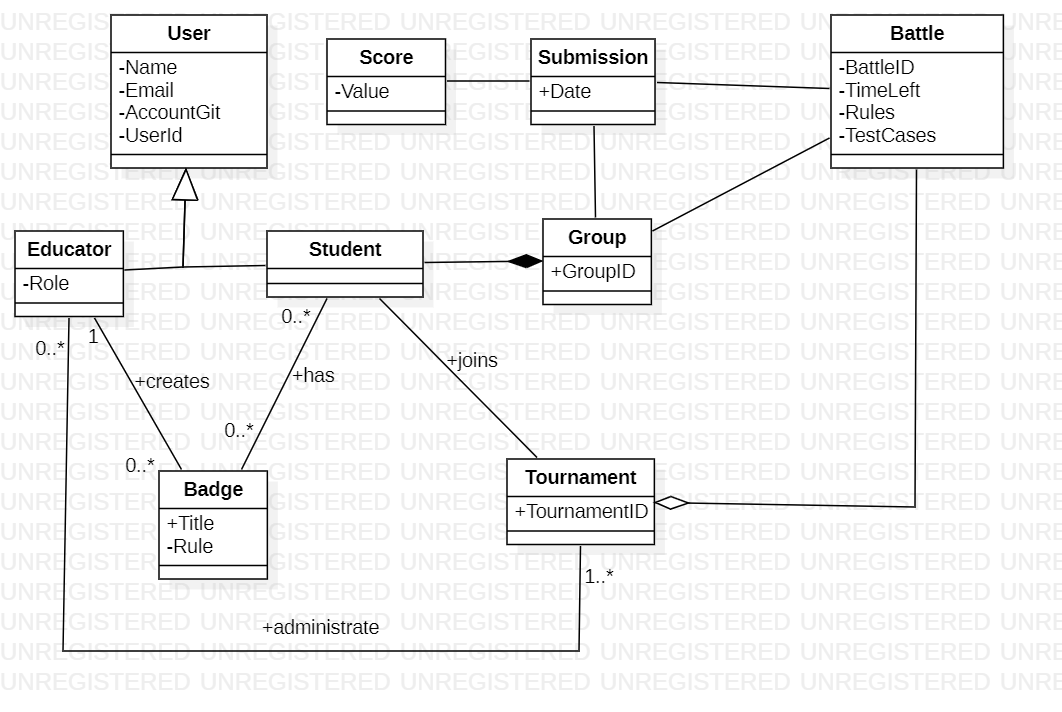
\includegraphics[width=0.9\textwidth]{LaudiziMarusicMassarelli/RASD/uml2.png}
            \subsubsection{Activity diagrams}
            \todo{devo aggiungere submission???}

            The charts below show the most significant flows of the platform. 
                
                   \subsubsection*{Creation of a tournament:}
                   \todo{se la notifica di nuovo torneo arriva a tutti devo togliere invite participants?}
                $\\$
                $\\$
                        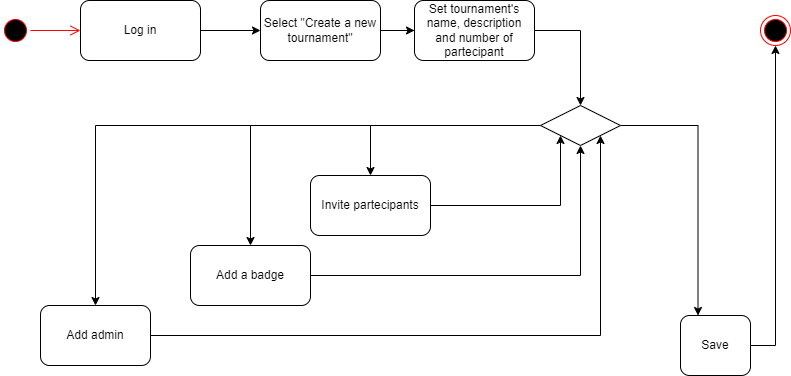
\includegraphics[width=0.9\textwidth]{LaudiziMarusicMassarelli/RASD/tournament.drawio.png}
                    \subsubsection*{Creation of a battle:} 
                    \todo{aggiungere il fatto che utente deve essere loggato}
                 $\\$
                  $\\$
                    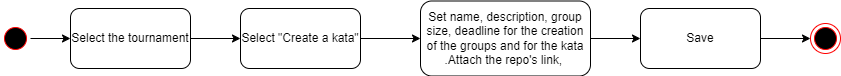
\includegraphics[width=0.9\textwidth]
            {LaudiziMarusicMassarelli/RASD/battle_creation.drawio.png}
            \subsubsection*{Creation of a group:}  
                 $\\$
                 If a user wants to create a new group, after selecting the kata he/she must select if the group will be public or private. Note that the system will check whether the maximum number of participant has been reached or not. 
                 $\\$
                  $\\$
                    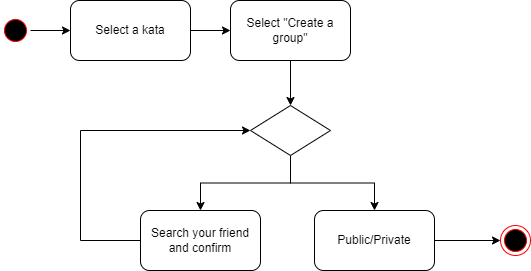
\includegraphics[width=0.9\textwidth]
            {LaudiziMarusicMassarelli/RASD/creationgroup.drawio.png}

            \subsubsection*{Join a group:}  
                 $\\$
                  $\\$
                    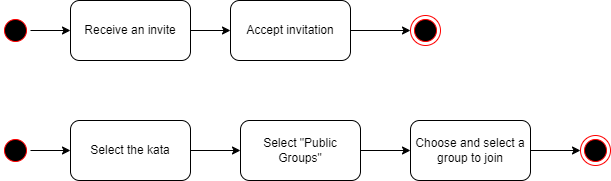
\includegraphics[width=0.9\textwidth]
            {LaudiziMarusicMassarelli/RASD/joinbattle.drawio.png}
            $\\$
             $\\$
                 There are two ways to join a group.
                  The user can simply accept a received invitation or select a kata and an open group to join. At the end of this procedure the system saves the changes to the group.
                    
           
        \subsection{Product functions}        
            \subsubsection{Sign-up and login}
                These functions will be accessible to all users. The sign-up feature enables users to register in the system. Specifically, each user will need to supply an email (which will serve as their username) and a password. Afterward, a verification email will be dispatched to the user. Once the user has confirmed their email, the system will prompt them to enter their personal information. If they are a regular user, they can also provide details about the vehicles they own. Conversely, if they are an operator, they must also provide information about the stations they own.
            \subsubsection{Create a tournament}
                Users acting as Admins can create a tournament and battles within them. A tournament can be public or private and admins have the privilege to invite participants and collaborators.
            
        \subsubsection{Join a battle}
            After a battle has been created, students utilize the platform to assemble teams for that specific battle. Each student has the option to participate individually in a battle or invite other students to join, adhering to the predetermined minimum and maximum number of students per group established for that battle. When the registration deadline expires, the platform will automatically generate a GitHub repository containing the code kata and subsequently send the repository link to all students who are members of the registered teams. At this stage, students are free to commence their work on the project.

        
            \subsubsection{Run tests}
                Each git push, performed on the challenge repository by a \group participating in the kata battle, triggers the platform that builds the project and runs the tests .
                \todo{where and how are the test ran?}

            \subsubsection{Assign score}
                After the submission has undergone testing, the system assigns a score to it. When the submission deadline expires, the kata battle enters in a consolidation stage where the \admins can review the repositories and perform further evaluations manually. When this stage finishes all participants in the battle are notified when the final battle rank becomes available.
                         
            \subsubsection{Create Badge}
                The system allows \admins of a tournament to create badges. In order to create a new badge the admin has to write a formula that involves variables provided by the system and set how long they last. During battles, the system checks to see if groups have met their goals, and if so, gives them the badges. Badges can be visualized by all users.

    \subsection{User characteristics}\label{sec:user_characteristics}
    The systems is built so that there are 2 types of users that interact with it: admins \& participants.
    Whichever \user can be both a participant or an admin depending on its role in the specific tournament. In detail:
        \begin{itemize}
        \item Admins use the platform to challenge participants by creating code
            kata battles in which groups of participants can compete against each other, thus proving (and improving) their skills.
        \item Participants are the ones who join groups to compete in the battles and use the system to improve their software development skills by training and challenging themselves.
        \end{itemize}
   
    \subsection{\hl{Assumptions, dependencies and constraints}}
    The following are the assumptions made for the domain. Such assumptions are properties and/or conditions that the system takes for granted, mostly because they are out of the control of the system itself, and hence need to be verified to assure the correct behavior of CodeKataBattles.
        \begin{enumerate}[label=\textbf{D\arabic*}:, left=0pt]
            \item User must have an internet connection
            \item User must have a GitHub account
            \item Each user must have one and only one account
            \item Each user must have a device to use the system
            \item Groups remain the same for the duration of the all tournament
            \item Users must have their personal e-mail where all the notifications can be sent
            \item A group in a battle is allowed to consist of just one person
            \item \hl{During a battle student pushes correctly his code in the branch of group inside the repository whose link is provided by the system.}
        \end{enumerate}

\section{Specific requirements}
    Here we include more details on all aspects in Section 2 if they can be useful for the development team.
    \subsection{External Interface Requirements}
        \subsubsection{User interfaces}
        \subsubsection{Hardware interfaces}
            This system is meant to interface only with software.
        \subsubsection{Software interfaces}
            The system interacts with GitHub through the GitHub REST API, which supports a variety of HTTP methods, including POST and GET.      
        \subsubsection{Communication interfaces}
            The system uses the HTTPS protocol to transmit data over the internet.
    \subsection{Functional requirements}
    \todo {Use case diagram}
        use case diagrams, use cases and related sequence and activity diagrams, and mapping on requirements

        \begin{enumerate}[label=\textbf{UC\arabic*}:]
        \item \textbf{Login}
        \begin{center}
            \begin{tabular}{ | m{8em} | m{10cm}|  } 
            \hline 
            \textbf{Name} & Login\\[1ex] 
            \hline 
            \textbf{Actors} & User \\[1ex] 
            \hline 
            \textbf{Entry condition} & The user has opened the CodeKataBattle website\\[1ex] 
            \hline \textbf{Event flow} & \begin{enumerate}[label=\textbf{\arabic*}:]
                \item The user inserts his username and password in the form
                \item The user clicks on the “Login” button
                \item The system checks the credentials
                \item The application shows the proper dashboard
                \end{enumerate} \\[1ex]
            \hline \textbf{Exit condition} & The user has access to the services for the right interface provided by CodeKataBattle \\[1ex]
            \hline \textbf{Exception} & \textbf{(3)} The data inserted are not valid. The system returns to the entry condition. \\[1ex]
            \hline
\end{tabular}
\captionof{table}{Login}
\end{center}

    \item \textbf{Sign-up}
    \begin{center}
        \begin{tabular}{ | m{8em} | m{10cm}|  } 
            \hline 
            \textbf{Name} & Sign-up\\[1ex] 
            \hline 
            \textbf{Actors} & Guest \\[1ex] 
            \hline 
            \textbf{Entry condition} & A person has downloaded the website and has a working internet connection \\[1ex] 
            \hline 
            \textbf{Event flow} & \begin{enumerate}[label=\textbf{\arabic*}:]
                \item Clicks on “Register”
                \item Inserts his data and fills mandatory fields
                \item Account is registered by the system
            \end{enumerate} \\[1ex]
            \hline 
            \textbf{Exit condition} & The guest is now registered into the system and becomes a User \\[1ex]
            \hline 
            \textbf{Exception} & \textbf{(2)} Email is already associated with another account, User was already registered in the system \\[1ex]
            \hline
        \end{tabular}
        \captionof{table}{Sign-up}
    \end{center}

    \item \textbf{Create a tournament}
    \begin{center}
        \begin{tabular}{ | m{8em} | m{10cm}|  } 
            \hline 
            \textbf{Name} & Create a tournament\\[1ex] 
            \hline 
            \textbf{Actors} & Educator \\[1ex] 
            \hline 
            \textbf{Entry condition} & The admin is logged in and has a working internet connection  \\[1ex] 
            \hline 
            \textbf{Event flow} & \begin{enumerate}[label=\textbf{\arabic*}:]
                \item Visits the "home" pages
                \item Clicks on “Create new tournament”
                \item Inserts tournament name and duration and invites other colleagues as collaborators in the tournament.
                \item Tournament is registered by the system
            \end{enumerate} \\[1ex]
            \hline 
            \textbf{Exit condition} & The tournament is now registered into the system, a notification is sent to all students which can now subscribe  \\[1ex]
            \hline 
            \textbf{Exception} & \textbf{(3)} Colleague is not registered \\[1ex]
            \hline 
        \end{tabular}
        \captionof{table}{Create tournament}
    \end{center}
       

        \item \textbf{Create a battle}
    \begin{center}
        \begin{tabular}{ | m{8em} | m{10cm}|  } 
            \hline 
            \textbf{Name} & Create a battle\\[1ex] 
            \hline 
            \textbf{Actors} & Admin \\[1ex] 
            \hline 
            \textbf{Entry condition} & The admin is logged in and has a working internet connection  \\[1ex] 
            \hline 
            \textbf{Event flow} & \begin{enumerate}[label=\textbf{\arabic*}:]
                \item Admin clicks on the tournament for which a battle needs to be added from the home page
                \item Clicks on “Add a new battle”
                \item Inserts the description and software project (including test cases and build automation scripts),sets the minimum and maximum number of students per group, the registration deadline and the final submission deadline and finally clicks on "Create"
                \item Battle is registered by the system
            \end{enumerate} \\[1ex]
            \hline 
            \textbf{Exit condition} & The battle is now registered into the system, and  and a notification is sent to all students in the tournament\\[1ex]
            \hline 
    
        \end{tabular}
        \captionof{table}{Create a battle}
    \end{center}
        \item \textbf{Join a tournament}
             \begin{center}
        \begin{tabular}{ | m{8em} | m{10cm}|  } 
            \hline 
            \textbf{Name} & Join a tournament\\[1ex] 
            \hline 
            \textbf{Actors} & Groups \\[1ex] 
            \hline 
            \textbf{Entry condition} & The student is logged in and has a working internet connection \\[1ex] 
            \hline 
            \textbf{Event flow} & \begin{enumerate}[label=\textbf{\arabic*}:]
                \item Student receives notification of the newly created tournament
                \item Clicks on "Join tournament" from its home page
            \end{enumerate} \\[1ex]
            \hline 
            \textbf{Exit condition} & Student is successfully subscribed to the tournament\\[1ex]
            \hline
            \textbf{Exception} & \textbf{(2)} The registration deadline is expired\\[1ex]
            \hline 
        \end{tabular}
        \captionof{table}{Join a tournament}
    \end{center}
    
        \item \textbf{Join a battle}
             \begin{center}
        \begin{tabular}{ | m{8em} | m{10cm}|  } 
            \hline 
            \textbf{Name} & Join a battle\\[1ex] 
            \hline 
            \textbf{Actors} & Groups and Student \\[1ex] 
            \hline 
            \textbf{Entry condition} & Each one in the group has an CodeKataBattle account and is subscribed to a tournament \\[1ex] 
            \hline 
            \textbf{Event flow} & \begin{enumerate}[label=\textbf{\arabic*}:]
                \item Student receives notification of the newly created battle.  
                \item Reaches the tournament page either by clicking on the notification or selecting the tournament from his home page.
                \item Clicks on the "Join battle" button.
                \item Either creates a new group and optionally invites his friends or joins an existing group.
            \end{enumerate} \\[1ex]
            \hline 
            \textbf{Exit condition} & The system has recorded the group's registration, and it is  pending approval from all the invited members of the group \\[1ex]
            \hline
            \textbf{Exception} & \textbf{(2)} The registration deadline is expired \\
                                & \textbf{(3)} The invited student doesn't exist (is not registered in the platform)\\[1ex]
            \hline 

        \end{tabular}
        \captionof{table}{Join a battle}
        \end{center}





        
        \item \textbf{Join a group}
            \begin{center}
        \begin{tabular}{ | m{8em} | m{10cm}|  } 
            \hline 
            \textbf{Name} & Join a group\\[1ex] 
            \hline 
            \textbf{Actors} & Student, Group\\[1ex] 
            \hline 
            \textbf{Entry condition} & The student is logged in and has a working internet connection. He receives the notification of an invite. \\[1ex] 
            \hline 
            \textbf{Event flow} & \begin{enumerate}[label=\textbf{\arabic*}:]
                \item Student sees the notification from his personal page.
                \item Student clicks on the notification.
                \item Student clicks on enter the group button of the notification.
                \item The System takes the student to the battle page 
            \end{enumerate} \\[1ex]
            \hline 
            \textbf{Exit condition} & Student is successfully in the group.\\[1ex]
            \hline
            \textbf{Exception} & \textbf{(1)} The registration deadline is expired. In this case, the system prompts on the screen that the student is late, and nothing else happens.\\[1ex]
            \hline
            \textbf{Exception} & \textbf{(2)} The student is not in the same tournament as the sender of the notification. In this case, the student is asked to join the tournament first.\\[1ex]
            \hline 
        \end{tabular}
    \end{center}


        
        \begin{center}
        \begin{tabular}{ | m{8em} | m{10cm}|  } 
            \hline 
            \textbf{Name} & Join a group\\[1ex] 
            \hline 
            \textbf{Actors} & Student, Group\\[1ex] 
            \hline 
            \textbf{Entry condition} & The student is logged in and has a working internet connection. He receives the notification of an invite. \\[1ex] 
            \hline 
            \textbf{Event flow} & \begin{enumerate}[label=\textbf{\arabic*}:]
                \item Student sees the notification from his personal page.
                \item Student clicks on the notification.
                \item Student clicks on reject button of the notification.
                \item The System prompts on the screen that the student rejected the invitation. 
            \end{enumerate} \\[1ex]
            \hline 
            \textbf{Exit condition} & Student is not in the group, the sender of the notification is notified of the refusal.\\[1ex]
            \hline
        \end{tabular}
        \end{center}


        \begin{center}
        \begin{tabular}{ | m{8em} | m{10cm}|  } 
            \hline 
            \textbf{Name} & Join a group\\[1ex] 
            \hline 
            \textbf{Actors} & Student, Group\\[1ex] 
            \hline 
            \textbf{Entry condition} & The student is logged in and has a working internet connection. He is a participant to a tournament, clicks the join battle button from the tournament page.  \\[1ex]
            \hline 
            \textbf{Event flow} & \begin{enumerate}[label=\textbf{\arabic*}:]
                \item Student is in the join battle page.
                \item Student looks for an open group that is incomplete.
                \item Student clicks on the selected group.
            \end{enumerate} \\[1ex]
            \hline 
            \textbf{Exit condition} & Student is successfully a participant of the group.\\[1ex]
            \hline 
        \end{tabular}
        \end{center}










        
        \item create a group
            \begin{center}
            \begin{tabular}{ | m{8em} | m{10cm}|  } 
            \hline 
            \textbf{Name} & Create a group\\[1ex] 
            \hline 
            \textbf{Actors} & Student, Group\\[1ex] 
            \hline 
            \textbf{Entry condition} & The student is logged in and has a working internet connection. He is a participant in a tournament, he clicked on the join button of a battle. \\[1ex] 
            \hline 
            \textbf{Event flow} & \begin{enumerate}[label=\textbf{\arabic*}:]
                \item The Student clicks on the create group button.
                \item The Student can either invite other students or not.
                \item The Student choose to make the group open or closed.
            \end{enumerate} \\[1ex]
            \hline 
            \textbf{Exit condition} & Student is successfully in the group and eventual invitations to other students are sent.\\[1ex]
            \hline
            \end{tabular}
            \end{center}



        \item accept or reject the invitation to an admin group
            \begin{center}
            \begin{tabular}{ | m{8em} | m{10cm}|  } 
            \hline 
            \textbf{Name} & Accept the invitation to admin group\\[1ex] 
            \hline 
            \textbf{Actors} & Teacher, Admin group\\[1ex] 
            \hline 
            \textbf{Entry condition} & The Teacher is logged in and has a working internet connection. He/she received the notification of an invitation to an admin group. \\[1ex] 
            \hline 
            \textbf{Event flow} & \begin{enumerate}[label=\textbf{\arabic*}:]
                \item The teacher sees the notification from his/hers personal page.
                \item The teacher clicks on the notification.
                \item The teacher clicks on the accept button of the notification.
                \item The System prompts on the screen that the teacher accepted the invitation. 
            \end{enumerate} \\[1ex]
            \hline 
            \textbf{Exit condition} & The teacher is in the admin group.\\[1ex]
            \hline
            \textbf{Exception} & The tournament is not active anymore. The screen prompts an information message and nothing else happens.\\[1ex]
            \hline 
            \end{tabular}
            \end{center}



            \begin{center}
            \begin{tabular}{ | m{8em} | m{10cm}|  } 
            \hline 
            \textbf{Name} & Reject the invitation to admin group\\[1ex] 
            \hline 
            \textbf{Actors} & Teacher, Admin group\\[1ex] 
            \hline 
            \textbf{Entry condition} & The Teacher is logged in and has a working internet connection. He/she received the notification of an invitation to an admin group. \\[1ex] 
            \hline 
            \textbf{Event flow} & \begin{enumerate}[label=\textbf{\arabic*}:]
                \item The teacher sees the notification from his/hers personal page.
                \item The teacher clicks on the notification.
                \item The teacher clicks on the reject button of the notification.
                \item The System prompts on the screen that the teacher rejected the invitation. 
            \end{enumerate} \\[1ex]
            \hline 
            \textbf{Exit condition} & The teacher is in not in the admin group.\\[1ex]
            \hline
            \end{tabular}
            \end{center}


            
            
        \item create a badge



           \begin{center}
        \begin{tabular}{ | m{8em} | m{10cm}|  } 
            \hline 
            \textbf{Name} & Create a badge\\[1ex] 
            \hline 
            \textbf{Actors} & Teacher\\[1ex] 
            \hline 
            \textbf{Entry condition} & The teacher is logged in and has a working internet connection. He/she is an admin in a tournament. \\[1ex] 
            \hline 
            \textbf{Event flow} & \begin{enumerate}[label=\textbf{\arabic*}:]
                \item Teacher clicks on the edit tournament section.
                \item Teacher chooses if the badge is of type top or Boolean.
                \item Teacher writes a formula in the formula section using the variables available, visible on the screen.
                \item In case the formula is of type Boolean the teacher chooses how many participant can receive the badge.
                \item Teacher saves changes.
            \end{enumerate} \\[1ex]
            \hline 
            \textbf{Exit condition} & The system creates the badge and evaluates it on the tournament.\\[1ex]
            \hline
            \textbf{Exception} & The formula is always false or always true, so the system reject the changes and prompts on the screen an informative message. \\[1ex]
            \hline 
        \end{tabular}
    \end{center}




        
        \item push the code on GitHub

            
               \begin{center}
        \begin{tabular}{ | m{8em} | m{10cm}|  } 
            \hline 
            \textbf{Name} & Push the code on GitHub\\[1ex] 
            \hline 
            \textbf{Actors} & Student, GitHub repository\\[1ex] 
            \hline 
            \textbf{Entry condition} & The student is logged in and has a working internet connection. He/she is a participant to a tournament, is currently in a battle, received the link to the repository and forked the repository. \\[1ex] 
            \hline 
            \textbf{Event flow} & \begin{enumerate}[label=\textbf{\arabic*}:]
                \item Student pushes on the main branch of his group fork.
                \item The GitHub action provided in the repository notifies the system of the push.
                \item The system runs test on the code.
                \item A score is provided based on the system performances.
                \item If any push has been performed before and the new score surpasses the old one, the points that were given are revoked and the new points are assigned to each one of the group members.
            \end{enumerate} \\[1ex]
            \hline 
            \textbf{Exit condition} & The system updates the points and consequently the leaderboard.\\[1ex]
            \hline
            \textbf{Exception} & The battle expired so the code is not evaluated and no points are assigned to the group.\\[1ex]
            \hline 
        \end{tabular}
    \end{center}


        
        \item visualize tournaments in which you are an admin



      \begin{center}
        \begin{tabular}{ | m{8em} | m{10cm}|  } 
            \hline 
            \textbf{Name} & Visualize the tournaments in which you are an admin\\[1ex] 
            \hline 
            \textbf{Actors} & Teacher, Admin\\[1ex] 
            \hline 
            \textbf{Entry condition} & The teacher is logged in and has a working internet connection. \\[1ex] 
            \hline 
            \textbf{Event flow} & \begin{enumerate}[label=\textbf{\arabic*}:]
                \item The teacher goes to his/hers home page.
            \end{enumerate} \\[1ex]
            \hline 
            \textbf{Exit condition} & Only the tournaments where he/she is an admin are showed.\\[1ex]
        \end{tabular}
    \end{center}


        
        \item visualize tournaments in which you are a participant
            \begin{center}
            \begin{tabular}{ | m{8em} | m{10cm}|  } 
                \hline 
                \textbf{Name} & Visualize the tournaments in which you are a participant\\[1ex] 
                \hline 
                \textbf{Actors} & Student, Participant\\[1ex] 
                \hline 
                \textbf{Entry condition} & The student is logged in and has a working internet connection. \\[1ex] 
                \hline 
                \textbf{Event flow} & \begin{enumerate}[label=\textbf{\arabic*}:]
                    \item The student goes to his/hers home page.
                \end{enumerate} \\[1ex]
                \hline 
                \textbf{Exit condition} & Both the tournaments where he/she is a participant and the ones where he/she participates are showed.\\[1ex]
            \end{tabular}
            \end{center}




    
        \item Visualize tournaments where you are neither a participant neither an admin
                 $\\$
            \begin{center}
                \begin{tabular}{ | m{8em} | m{10cm}|  } 
                \hline 
                \textbf{Name} & Visualize tournaments where you are neither a participant neither an admin\\[1ex] 
                \hline 
                \textbf{Actors} & User \\[1ex] 
            \hline 
            \textbf{Entry condition} & The user is correctly logged in and has working internet connection  \\[1ex] 
            \hline \textbf{Event flow} & \begin{enumerate}[label=\textbf{\arabic*}:]
                \item Visits the "home" page
                \end{enumerate} \\[1ex]
             \hline \textbf{Exit condition} & The user can correctly visualize on the screen all the disposable tournaments \\[1ex]
            \hline 
\end{tabular}
\end{center}
        \item Visualize the participants of a tournament
           $\\$
            \begin{center}
                \begin{tabular}{ | m{8em} | m{10cm}|  } 
                \hline 
                \textbf{Name} & Visualize the participant of a tournament\\[1ex] 
                \hline 
                \textbf{Actors} & User \\[1ex] 
            \hline 
            \textbf{Entry condition} & The user is correctly logged in and has working internet connection  \\[1ex] 
            \hline \textbf{Event flow} & \begin{enumerate}[label=\textbf{\arabic*}:]
                \item Visits the "home" pages
                \item Select a tournament
                \end{enumerate} \\[1ex]
            \hline \textbf{Exit condition} & The participants of the selected tournament are visible now on the screen \\[1ex]
            \hline
\end{tabular}
\end{center}
        \item Visualize an user details
                 $\\$
            \begin{center}
                \begin{tabular}{ | m{8em} | m{10cm}|  } 
                \hline 
                \textbf{Name} & Visualize an user details\\[1ex] 
                \hline 
                \textbf{Actors} & User \\[1ex] 
            \hline 
            \textbf{Entry condition} & The user is correctly logged in and has working internet connection  \\[1ex] 
            \hline \textbf{Event flow} & \begin{enumerate}[label=\textbf{\arabic*}:]
                \item Visits the "home" pages
                \item Select a tournament
                \item Select a user from the rank or from group settings
                \end{enumerate} \\[1ex]
            \hline \textbf{Exit condition} & The system shows on the screen the user's details including name, user ID and badges \\[1ex]
            \hline
\end{tabular}
\end{center}
        \item Visualize the battle instructions
                        $\\$
            \begin{center}
                \begin{tabular}{ | m{8em} | m{10cm}|  } 
                \hline 
                \textbf{Name} & Visualize the battle instructions\\[1ex] 
                \hline 
                \textbf{Actors} & User \\[1ex] 
            \hline 
            \textbf{Entry condition} & The user is correctly logged in and has a working internet connection  \\[1ex] 
            \hline \textbf{Event flow} & \begin{enumerate}[label=\textbf{\arabic*}:]
                \item Visits the "home" pages
                \item Select a tournament
                \item Select a battle
                \end{enumerate} \\[1ex]
            \hline \textbf{Exit condition} & The system shows on the screen all the battle's details \\[1ex]
            \hline
\end{tabular}
\end{center}
        \item Add an admin
                   $\\$
            \begin{center}
                \begin{tabular}{ | m{8em} | m{10cm}|  } 
                \hline 
                \textbf{Name} & Add an admin\\[1ex] 
                \hline 
                \textbf{Actors} & Admin, Educator\\[1ex] 
            \hline 
            \textbf{Entry condition} & The admin is correctly logged in and has a working internet connection  \\[1ex] 
            \hline \textbf{Event flow} & \begin{enumerate}[label=\textbf{\arabic*}:]
                \item Visits the "home" pages
                \item Select one of the tournament in "Managing" area.
                \item Select "Edit settings".
                \item Select "Add admin".
                \item Insert educator's ID.
                \item Commit the changes.
                \end{enumerate} \\[1ex]
            \hline \textbf{Exit condition} & The system correctly added the user to the list of admin and gave him/her all the admin's privileges \\[1ex]
            \hline \textbf{Exception} & \textbf{(5)} User is not registered \\[1ex]
            \hline
\end{tabular}
\end{center}
        \item Modify group settings
                  $\\$
            \begin{center}
                \begin{tabular}{ | m{8em} | m{10cm}|  } 
                \hline 
                \textbf{Name} & Modify group settings\\[1ex] 
                \hline 
                \textbf{Actors} & Participant \\[1ex] 
            \hline 
            \textbf{Entry condition} & The participant is correctly logged and is registered to a tournament  \\[1ex] 
            \hline \textbf{Event flow} & \begin{enumerate}[label=\textbf{\arabic*}:]
                \item Visits the "home" pages
                \item Select one of the tournament in "Participant" area.
                \item Select a battle in the tournament.
                \item Select "Group settings".
                \item The participant can add other participants or change the group's visibility.
                \item Commit the changes.
                \end{enumerate} \\[1ex]
            \hline \textbf{Exit condition} & The system correctly saved the changes.\\[1ex]
            \hline \textbf{Exception} & \textbf{(5)} The changes does not respect the number of participants constraint or the searched participant does not exist. \\[1ex]
            \hline
\end{tabular}
\end{center}
        \end{enumerate}
       \subsubsection{Sequence diagrams}
             \begin{figure}[!ht]
                \centering
                
\includegraphics[width=2cm]{LaudiziMarusicMassarelli/RASD/white.jpg}
                \label{fig:white}
            \end{figure}
       
            \begin{figure}[!ht]
                \centering
                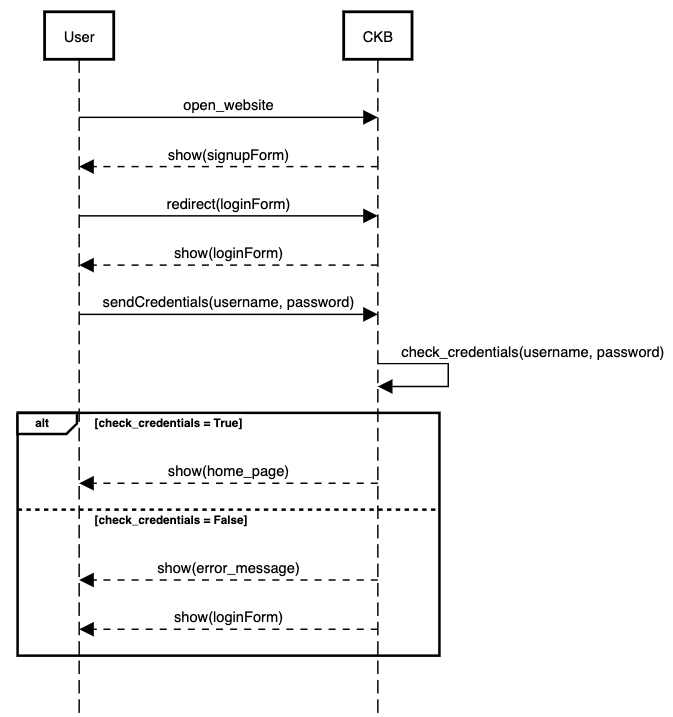
\includegraphics[width=16cm]{LaudiziMarusicMassarelli/RASD/LoginSD.png}
                \caption{User Login}
                \label{fig:login}
            \end{figure}

            \begin{figure}[!ht]
                \centering
                
\includegraphics[width=5cm]{LaudiziMarusicMassarelli/RASD/white.jpg}
                \label{fig:white}
            \end{figure}
        
            \begin{figure}[!ht]
                \centering
                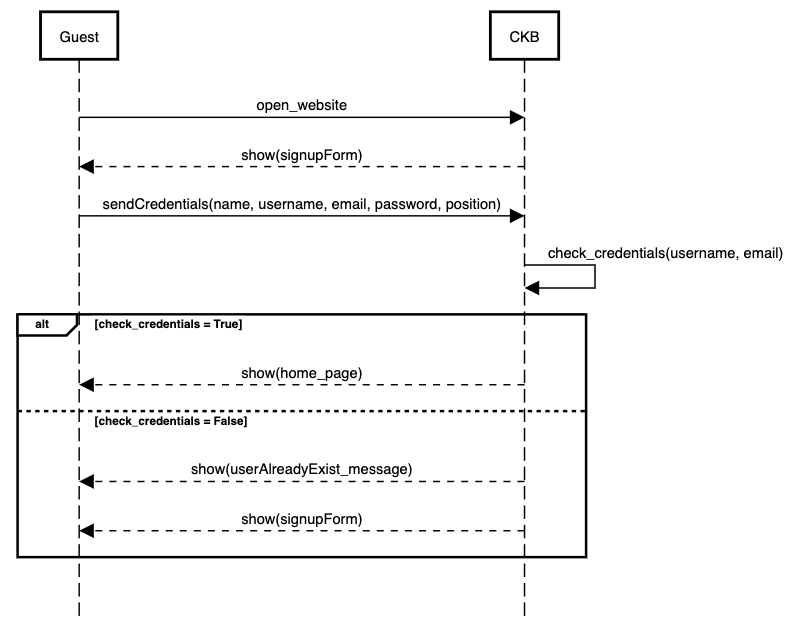
\includegraphics[width=13cm]{LaudiziMarusicMassarelli/RASD/SignupSD.png}
                \caption{Guest Login}
                \label{fig:login}
            \end{figure}

            \begin{figure}[!ht]
                \centering
                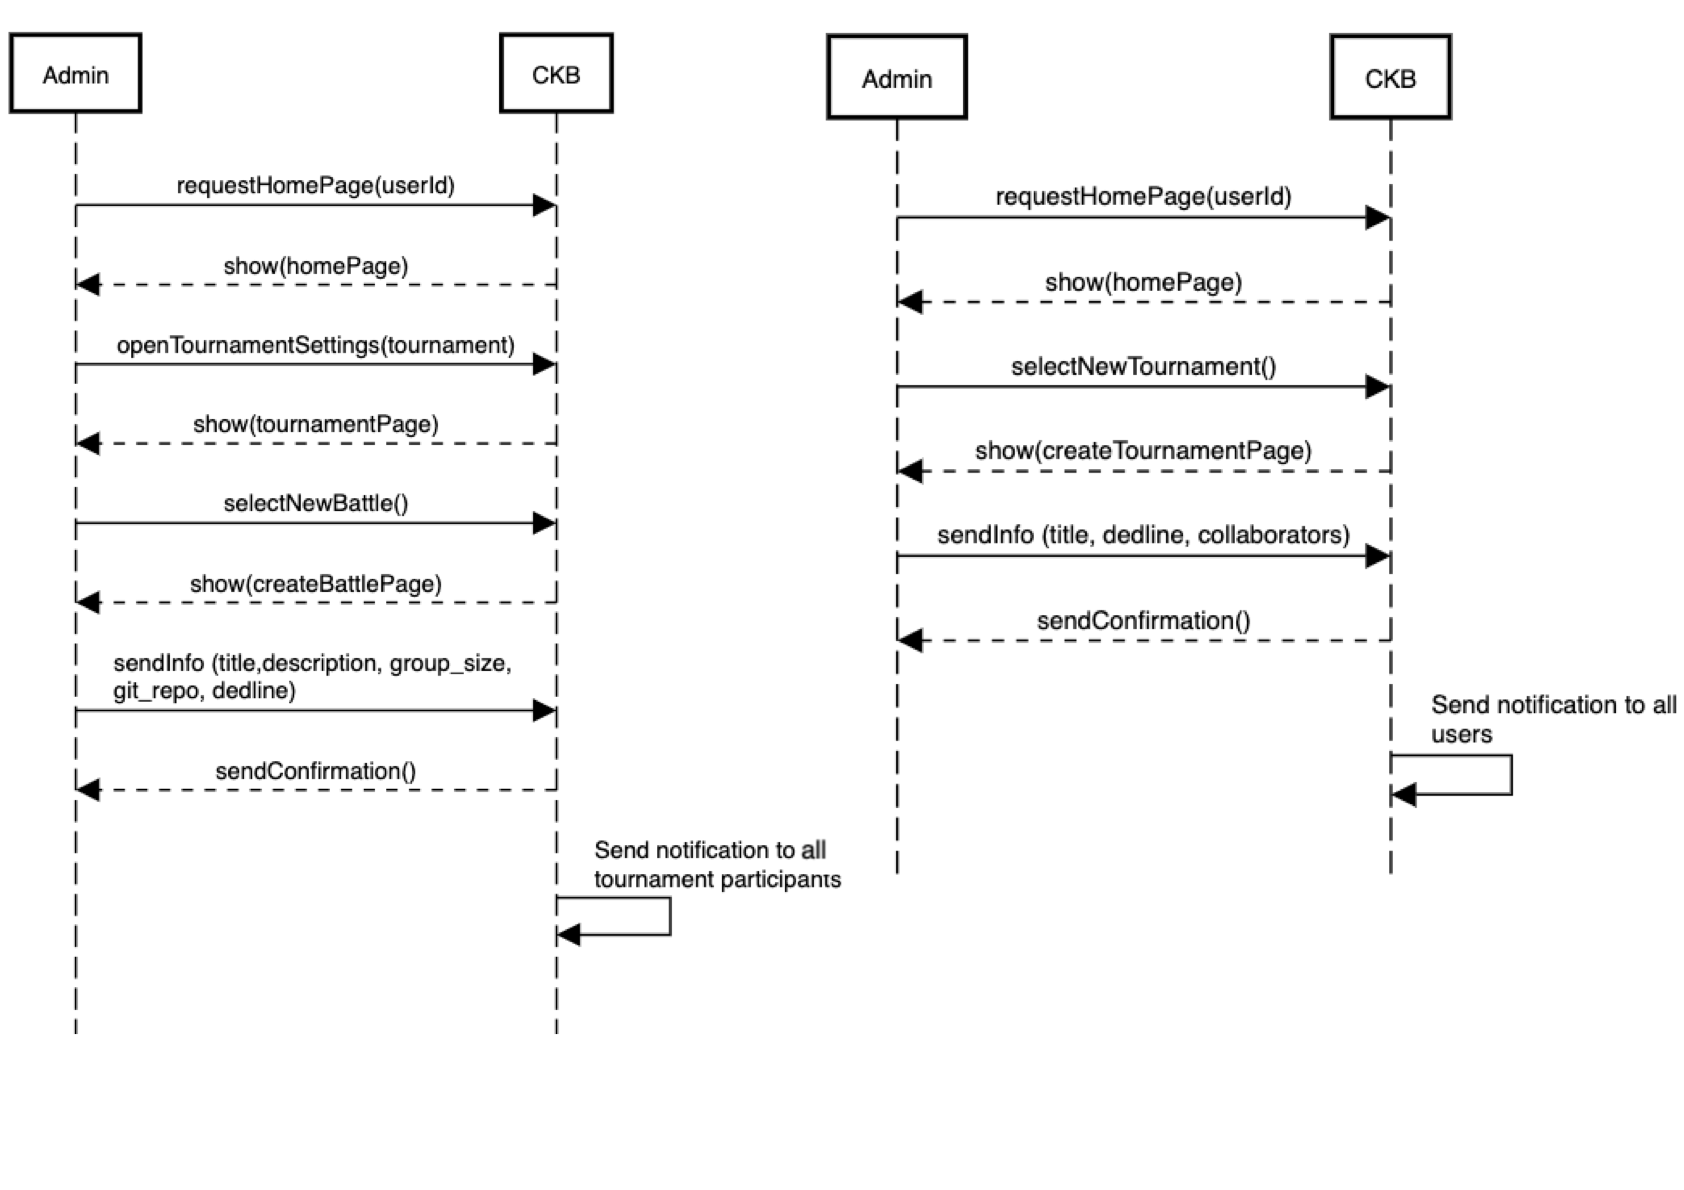
\includegraphics[width=15cm]{LaudiziMarusicMassarelli/RASD/create.png}
                \caption{Create new battle \& Create new tournament}
                \label{fig:create}
            \end{figure}

            \begin{figure}[!ht]
                \centering
                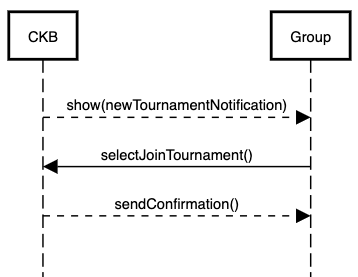
\includegraphics[width=10cm]{LaudiziMarusicMassarelli/RASD/JoinTournament.png}
                \caption{Join tournament}
                \label{fig:join Tournament}
            \end{figure}
            
            \begin{figure}[!ht]
                \centering
                
\includegraphics[width=5cm]{LaudiziMarusicMassarelli/RASD/white.jpg}
                \label{fig:white}
            \end{figure}
             
            \begin{figure}[!ht]
                \centering
                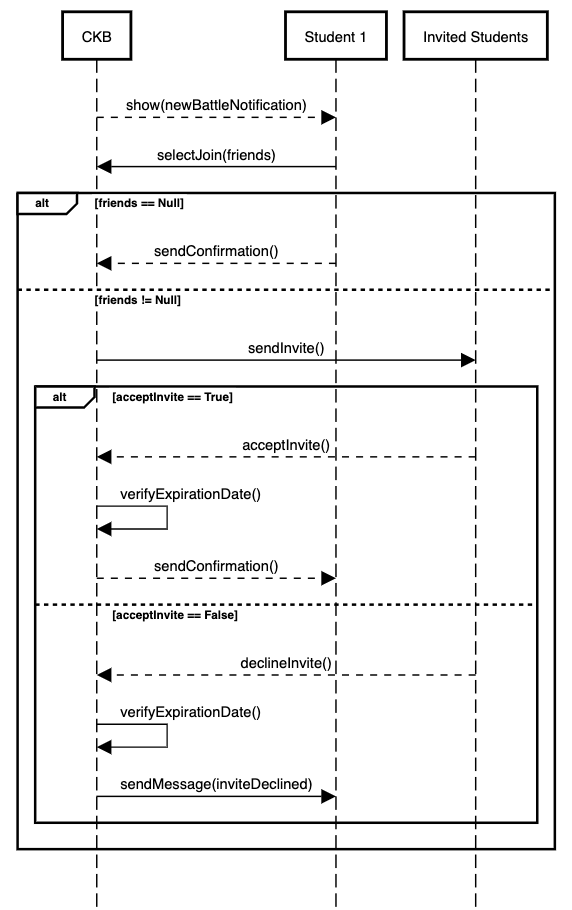
\includegraphics[width=10cm]{LaudiziMarusicMassarelli/RASD/joinBalltle.png}
                \caption{Join Battle}
                \label{fig:join Battle}
            \end{figure}
            

\begin{figure}[!ht]
    \centering
    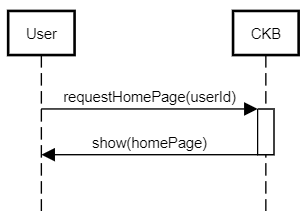
\includegraphics[width=7cm]{LaudiziMarusicMassarelli/RASD/VisualizeTournaments (1).png}
    \caption{Visualize tournaments when you are neither a participant neither an educator}
    \label{fig:Visualize tournaments when you are neither a participant neither an educator}
\end{figure}

\begin{figure}[!ht]
    \centering
    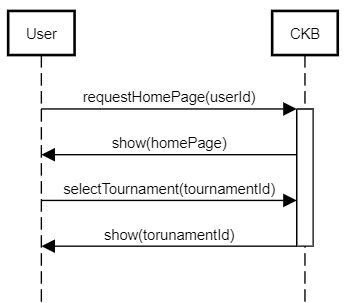
\includegraphics[width=8cm]{LaudiziMarusicMassarelli/RASD/Visualizeparticipants.png}
    \caption{Visualize the participants of a tournament}
    \label{fig:Visualize the participants of a tournament}
\end{figure}

\begin{figure}[!ht]
    \centering
    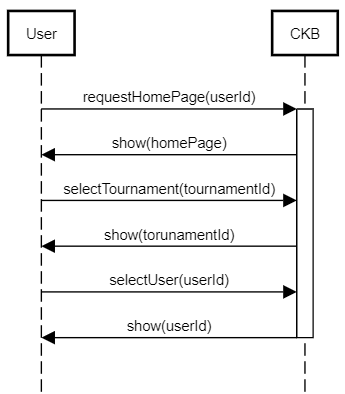
\includegraphics[width=8cm]{LaudiziMarusicMassarelli/RASD/VisualizeUser.png}
    \caption{Visualize a user's details}
    \label{fig:Visualize user's details}
\end{figure}

\begin{figure}[!ht]
    \centering
    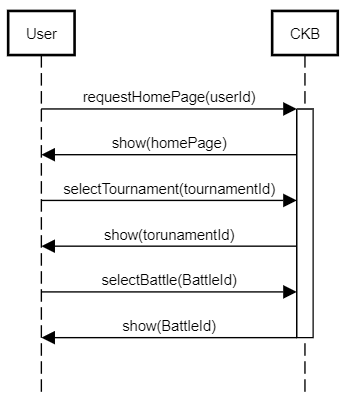
\includegraphics[width=8cm]{LaudiziMarusicMassarelli/RASD/VisualizeBattle.png}
    \caption{Visualize battle's instructions}
    \label{fig:Visualize battle's instructions}
\end{figure}

\begin{figure}[!ht]
    \centering
    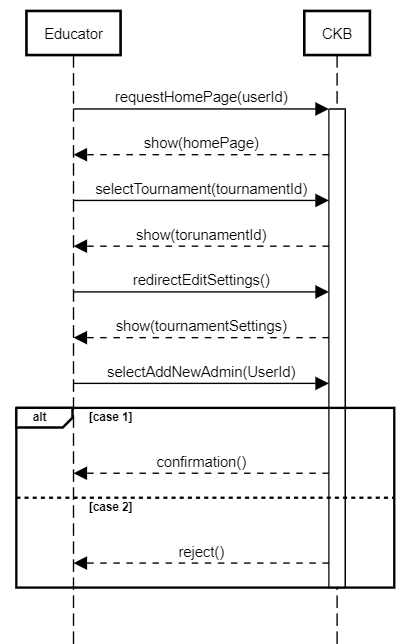
\includegraphics[width=8cm]{LaudiziMarusicMassarelli/RASD/AddAdmin (1).png}
    \caption{Add an educator}
    \label{fig:Add an educator}
\end{figure}

\begin{figure}[!ht]
    \centering
    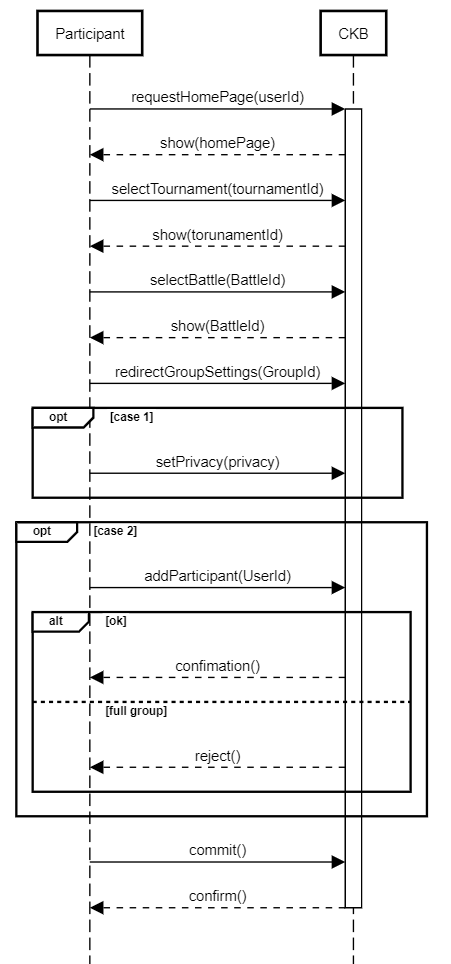
\includegraphics[width=8cm]{LaudiziMarusicMassarelli/RASD/modifygroup.png}
    \caption{Modify group settings}
    \label{fig:Modify group settings}
\end{figure}

$\\$
$\\$
    \subsection{Performance requirements}
    \subsection{Design Constraints}
        The system relies on internet connection to provide the service, if the internet infrastructure is slowed down or the user connection is poor the performances of the system will be compromised.
        \subsubsection{Standards compliance}
            General Data Protection Regulation (GDPR)
            The system has to adopt international standards about date and time use and representation.
        \subsubsection{Hardware limitations}
            The system to work needs all the users to have access to internet connection (2G/3G/4G/5G/Wi-Fi), a personal computer.
            
    \subsection{Software system attributes}
        \subsubsection{Reliability}
        To ensure the reliability of the CodeKataBattle (CKB) platform, it is imperative to establish regular data backup mechanisms and a robust error-handling system in order to minimize the impact of unforeseen crushes.
        \subsubsection{Availability}
        Ensuring high availability is a key consideration for the CKB platform. To achieve this, a redundancy system will be implemented. 
        \subsubsection{Security}
        The system will record some private informations so it is important to implement a secure platform. In particular, user's passwords and data should be encrypted in order to avoid to be changed or seen by malicious people.
        To safeguard sensitive communications, secure connections (HTTPS) will be enforced for all interactions.
        \subsubsection{Maintainability}
        Maintaining the CKB platform's codebase is vital for long-term success. For this reason it is important to comment and document the code. Unit and integration test must come along with every addition to the code and must cover at least 80\% of it. 
        \subsubsection{Portability}
        Achieving portability is a key design consideration for the CKB platform. The software should run on all the possible operating systems that supports a web browser.

$\\$
\todo{there can be multiple katas open at the same time}
{Evaluate Badges}
\todo {probably this section doesn't belong here}
\todo{how often are the badges checked? every commit? can the system identify when is sensible to check a badge based on the kind of badge?}

               \todo{where should this section go?}
                Scoring method (copy and paste of the instructions)
                The score is a natural number between 0 and 100 determined by considering some mandatory factors evaluated in a fully automated way, and optional factors evaluated manually by educators. Mandatory automated evaluation includes:
                • functional aspects, measured in terms of number of test cases that pass out of all test cases (the
                higher the better);
                • timeliness, measured in terms of time passed between the registration deadline and the last
                commit (the lower the better);
                • quality level of the sources, extracted through static analysis tools that consider multiple aspects
                such as security, reliability, and maintainability (the higher the better). Aspects are selected by the
                educator at battle creation time. Optional manual evaluation includes:
                • personal score assigned by the educator, who checks and evaluates the work done by students (the
                higher the better).
                The CKB platform automatically updates the battle score of a team as soon as new push actions on GitHub are performed            

                \subsubsection{Create a Kata Battle}
                The system allows \admins to create a Kata Battle
                \todo {define a kata battle}. The process involves asking a
                textual description of the problem to solve by the \groups and a software project with build automation scripts whose structure depends on the programming language of choice for the kata. This project must contain a set of test cases, otherwise it won't be possible to perform the evaluation of the submissions. 
                \todo {can katas allow for different programming languages?}.
                After that the system prompts for some configurations parameters for the kata, such as minimum and maximum number of students per group, a registration deadline, a final submission deadline
                and additional configurations for scoring
                \todo {pay attention to the fact that scoring criterion are different based on the kata, so are not a property of the tournament}\\

                When the system receives in input the data required it performs some validity checks
                \todo{what are the necessary validity checks? what can't be validated and so has to be put in the constraints?}.
                 Later, it will ask for confirmation and the kata will be created.
                \todo{ Notifications will be sent?}
\section{Formal analysis using alloy}
\subsubsection{Send notification}
                The system has the possibility of sending notification to \users. There are multiple kinds of notifications that serves the purpose of updating \users on the status of the tournaments they are involved in and updating them on incoming invitations in tournaments, group or invitations as collaborators in the \adminGroup.
            
            
                \paragraph{Tournament created}
                     When a tournament is created, if public
                     all students subscribed to the CKB platform are notified.

                \paragraph{Battle created}
                    When someone in the \adminGroup of a tournament creates a kata battle, every \participant of that tournament is notified.
                \paragraph*{Send link}
                    When the registration deadline expires and the platform creates the GitHub repository the system sends a notification containing the link to all \participants of that tournament.
                \paragraph*{End of battle}
                    Once the consolidation stage finishes, all students participating in the battle are notified with the updated ranks.
                
                \paragraph{Tournament closure}
                    \todo{when does a tournament finishes?}
                    when a tournament finishes all the \participants are notified

                \paragraph*{Invite}
                    \todo{this section isn't specifically required but it makes sense considering the fact that one can invite team members so you have to someway understand that you have been invited}
                    The invitations can be received in different cases
                    \begin {itemize}
                        \item an \user can be invited in a \group participating a tournament.
                        \item an user can be invited in a tournament.

                         \todo{ invito a battaglia, invito a torneo , invito a creare battaglie}
                    \end {itemize}

\section{Effort spent}
    Antonio Marusic\\
    section 1: 2h\\
    section 2: 2:30h\\


    
\end{document}